\chapter{DESENVOLVIMENTO}
\label{cap:desenvolvimento}

Este capítulo documenta o sistema desenvolvido. A Seção \ref{sec:apresentacao} apresenta uma visão geral da solução e a Seção \ref{sec:processo} descreve o processo de desenvolvimento adotado. As Seções \ref{sec:rf} a \ref{sec:historias} especificam os requisitos, os atores, as regras de negócio e as histórias de usuário. A Seção \ref{sec:bd} apresenta a modelagem de dados, a Seção \ref{sec:diagramas} reúne os diagramas estruturais e comportamentais, a Seção \ref{sec:implementacao} detalha a implementação de cada etapa e a Seção \ref{sec:prototipo} apresenta a interface. Por fim, a Seção \ref{sec:testes} descreve a estratégia de testes.

\section{Apresentação do Sistema}
\label{sec:apresentacao}

O sistema desenvolvido é um conjunto de dois fluxos de automação executados na plataforma n8n, apoiados por um servidor de modelos de linguagem local. O fluxo de validação lê os planos de ensino em PDF de uma pasta local, extrai e segmenta o texto de cada plano, solicita ao modelo de linguagem a avaliação dos critérios, aplica regras determinísticas sobre a resposta e grava o resultado de cada plano em um arquivo JSON, em outra pasta local. O fluxo do \textit{dashboard} lê esses arquivos e gera, a cada acesso, uma página HTML com os indicadores do lote, o detalhamento de cada plano e a exportação dos resultados em CSV.

A Figura \ref{fig:arquitetura} apresenta a arquitetura da solução. Os dois serviços próprios, n8n e Ollama, são executados em contêineres Docker orquestrados por um arquivo Docker Compose e se comunicam por uma rede interna. O Ollama tem acesso à GPU do computador hospedeiro, onde o modelo Qwen2.5 é carregado. Duas pastas do computador hospedeiro são montadas no contêiner do n8n: a pasta \texttt{planos}, repositório de entrada onde a coordenação deposita os PDFs, e a pasta \texttt{resultados}, onde o sistema grava as validações. Dessa forma, o sistema não depende de serviços externos nem de credenciais, e a implantação se resume a iniciar os contêineres, importar os fluxos e copiar os planos para a pasta de entrada. Até a penúltima iteração, a entrada e a saída usavam o Google Drive e o Google Sheets, acessados por OAuth 2.0. Essa configuração exigia, a cada implantação, criar um projeto no Google Cloud, ativar as APIs, configurar a tela de consentimento e cadastrar as credenciais no n8n, etapa apontada na revisão do orientador como complexa demais para a adoção do sistema, e por isso foi substituída pelo armazenamento local.

\begin{figure}[htbp]
\centering
\caption{Arquitetura do sistema}
\label{fig:arquitetura}
\begin{tikzpicture}[every node/.style={font=\footnotesize}]
  % Linha 1: entrada, validação e modelo
  \node[ext, text width=2.4cm] (drive) at (0,2) {Pasta \texttt{planos}\\\scriptsize PDFs dos planos};
  \node[caixa, text width=3.9cm] (wfval) at (5.4,2) {\textbf{Workflow de validação}\\\scriptsize busca, extração, segmentação, \textit{prompt}, interpretação e registro};
  \node[ia, text width=2.7cm] (llm) at (11.0,2) {\textbf{Ollama}\\\scriptsize Qwen2.5 7B (Q4\_K\_M)\\\texttt{/api/generate}};
  \node[caixa, text width=2.7cm, font=\scriptsize] (gpu) at (11.0,0.25) {GPU NVIDIA (6 GB)};

  % Linha 2: resultados e dashboard
  \node[ext, text width=2.4cm] (sheets) at (0,-1.4) {Pasta \texttt{resultados}\\\scriptsize um JSON por plano};
  \node[caixa, text width=3.9cm] (wfdash) at (5.4,-1.4) {\textbf{Workflow do \textit{dashboard}}\\\scriptsize leitura dos resultados, HTML e CSV};

  % Linha 3: usuário
  \node[caixa, text width=3.9cm] (user) at (5.4,-4.2) {Coordenação, NDE ou docente\\\scriptsize navegador \textit{web}};

  % Agrupamentos
  \begin{scope}[on background layer]
    \node[grupo, fit=(wfval)(wfdash), inner sep=10pt] (n8n) {};
    \node[grupo, fit=(llm)(gpu), inner sep=10pt] (oll) {};
    \node[draw, rounded corners=4pt, black!80, fit=(n8n)(oll), inner sep=8pt] (docker) {};
  \end{scope}
  \node[font=\scriptsize\bfseries, anchor=south] at (n8n.north) {Contêiner n8n};
  \node[font=\scriptsize\bfseries, anchor=south] at (oll.north) {Contêiner Ollama};
  \node[font=\scriptsize\bfseries, anchor=south west] at ([yshift=1mm]docker.north west) {Docker Compose -- rede interna \texttt{tc-network}};

  % Fluxos
  \draw[seta] (drive) -- node[rotulo, above]{1. lê PDFs} (wfval);
  \draw[seta] ([yshift=2.5mm]wfval.east) -- node[rotulo, above]{2. \textit{prompt} + esquema} ([yshift=2.5mm]llm.west);
  \draw[seta] ([yshift=-2.5mm]llm.west) -- node[rotulo, below]{3. JSON} ([yshift=-2.5mm]wfval.east);
  \draw[thick, dotted] (llm) -- (gpu);
  \draw[seta] (wfval.south west) -- node[rotulo, above, sloped]{4. um arquivo por plano} (sheets.north east);
  \draw[seta] (sheets) -- node[rotulo, above]{5. leitura} (wfdash);
  \draw[seta, {Stealth[length=2.2mm]}-{Stealth[length=2.2mm]}] (user) -- node[rotulo, right]{6. \texttt{GET /webhook/dashboard}} (wfdash);
\end{tikzpicture}

\legend{Fonte: Elaborado pelo autor (2026).}
\end{figure}

Três princípios orientaram o projeto. O primeiro é a divisão de trabalho entre regras e modelo: o que pode ser verificado de forma exata, como contar referências, é feito por código, e o LLM é reservado aos julgamentos que exigem interpretação. O segundo é a verificabilidade: cada critério recebe um status de um conjunto fechado e uma observação curta, e o \textit{dashboard} oferece acesso direto ao PDF original. O terceiro é o controle humano: o sistema faz uma triagem e não toma decisões, cabendo à coordenação e ao NDE confirmar ou descartar cada apontamento.

\section{Metodologia de desenvolvimento de software}
\label{sec:processo}

A solução apresentada na seção anterior não foi definida de uma só vez, mas construída ao longo de várias versões. O desenvolvimento seguiu um processo iterativo e incremental, no qual o sistema é construído em versões sucessivas e cada versão é avaliada antes de orientar a seguinte \cite{Sommerville2016, Pressman2016}. A escolha se justifica pelo caráter exploratório do projeto: não era possível prever, antes de executar o sistema sobre planos reais, como o modelo de linguagem se comportaria diante dos documentos, quais regras seriam ambíguas ou quais limites de infraestrutura seriam atingidos. Em linha com os valores do Manifesto Ágil \cite{Beck2001}, privilegiou-se ter software funcionando desde a primeira iteração e responder às mudanças identificadas nas execuções, em vez de seguir um plano fechado.

Cada iteração seguiu o mesmo ciclo: (i) executar a versão corrente sobre o corpus completo; (ii) inspecionar, nos resultados gravados e no histórico de execuções do n8n, os resultados e as falhas; (iii) identificar a causa raiz do problema mais grave; e (iv) implementar e documentar a correção. O código dos fluxos, exportado do n8n em formato JSON, e a configuração da infraestrutura foram versionados com Git em um repositório no GitHub, e um arquivo de documentação registrou as instruções de instalação e os problemas conhecidos com suas soluções. A Tabela \ref{tab:iteracoes} resume as iterações realizadas.

\begin{table}[H]
\centering
\caption{Iterações de desenvolvimento}
\label{tab:iteracoes}
\footnotesize
\begin{tabular}{@{}L{2.4cm}L{9.1cm}L{2.9cm}@{}}
\toprule
\rowcolor[HTML]{EFEFEF}
\textbf{Período} & \textbf{Principais entregas e correções} & \textbf{Execução de referência} \\ \midrule
Maio/2026 & Primeira versão do fluxo: busca no Drive, extração de texto, avaliação do plano pelo LLM e registro na planilha & 22/05: 86,2\% de ERRO \\
Julho/2026 & Critérios definidos com o orientador; segmentação do texto por seções; \textit{dashboard} HTML; suporte a GPU; documentação de instalação & 07/07: 3,4\% de ERRO \\
Agosto/2026 & Processamento em blocos com uma requisição por vez e retentativas; adoção do Qwen2.5 7B; correção do contexto máximo do modelo (de 4.096 para 12.288 \textit{tokens}) & 10/08: 69,0\%; 25/08: 49,1\% de ERRO \\
Setembro/2026 & Contagem determinística de referências; regras determinísticas para objetivos e status geral; remoção da exigência de interdisciplinaridade & 10/09: 0\%; 15/09: 17,2\% de ERRO \\
Outubro/2026 & Segmentação ancorada no início da linha; contexto de 8.192 \textit{tokens}; \textit{FlashAttention} e \textit{KV cache} em 8 bits; \textit{timeout} de 180 s & 19/10: 0\% de ERRO \\
Novembro/2026 & Armazenamento local: planos lidos de uma pasta e resultados gravados em arquivos JSON, em substituição ao Google Drive e ao Google Sheets; exportação em CSV e abertura do PDF pelo \textit{dashboard} & Teste funcional do fluxo, sem nova execução sobre o corpus \\ \bottomrule
\end{tabular}
\legend{Fonte: Elaborado pelo autor (2026), com base no histórico de execuções e na planilha de resultados.}
\end{table}

Os problemas encontrados em cada iteração e o efeito das correções são analisados na Seção \ref{sec:res-robustez}.

\section{Requisitos Funcionais}
\label{sec:rf}

Os requisitos funcionais descrevem os serviços que o sistema deve oferecer \cite{Sommerville2016}. Eles foram levantados a partir do processo manual de conferência e refinados ao longo das iterações. A Tabela \ref{tab:rf} apresenta os requisitos funcionais implementados.

\begin{table}[H]
\centering
\caption{Requisitos funcionais}
\label{tab:rf}
\footnotesize
\begin{tabular}{@{}L{1.1cm}L{13.3cm}@{}}
\toprule
\rowcolor[HTML]{EFEFEF}
\textbf{Nº} & \textbf{Descrição do Requisito Funcional} \\ \midrule
RF01 & O sistema deve ler os arquivos PDF de uma pasta local configurada, ignorando arquivos de outros tipos. \\
RF02 & O sistema deve extrair o texto de cada plano de ensino em PDF. \\
RF03 & O sistema deve segmentar o texto nas seções do plano: identificação, ementa, metodologia, procedimentos de avaliação, horário de atendimento, objetivo geral, objetivos específicos, conteúdo programático, cronograma, avaliações e referências. \\
RF04 & O sistema deve contar as referências básicas e complementares de cada plano. \\
RF05 & O sistema deve avaliar os doze critérios da Tabela \ref{tab:criterios}, atribuindo a cada um o status OK, INCOMPLETO ou AUSENTE e uma observação. \\
RF06 & O sistema deve calcular o status geral do plano (OK, PENDENTE ou REPROVADO) a partir dos status dos critérios. \\
RF07 & O sistema deve registrar o status ERRO e o motivo da falha quando não for possível avaliar um plano. \\
RF08 & O sistema deve gravar o resultado de cada plano em um arquivo na pasta de resultados, com data e hora da validação e o \textit{link} para o PDF original. \\
RF09 & O sistema deve executar a validação automaticamente uma vez por dia e permitir a execução manual. \\
RF10 & O sistema deve disponibilizar um \textit{dashboard} com o total de planos e as quantidades e percentuais de planos aprovados, pendentes e com problemas. \\
RF11 & O \textit{dashboard} deve exibir, para cada plano, o status e a observação de cada critério. \\
RF12 & O \textit{dashboard} deve permitir abrir o PDF original de cada plano. \\
RF13 & O sistema deve permitir trocar o modelo de linguagem utilizado, inclusive por um serviço externo. \\
RF14 & O \textit{dashboard} deve permitir exportar todos os resultados em formato CSV. \\ \bottomrule
\end{tabular}
\legend{Fonte: Elaborado pelo autor (2026).}
\end{table}

\section{Requisitos Não Funcionais}
\label{sec:rnf}

Enquanto os requisitos funcionais definem o que o sistema faz, os requisitos não funcionais expressam restrições e qualidades do sistema \cite{Sommerville2016}. Eles foram organizados segundo as características de qualidade da norma ISO/IEC 25010 \cite{ISO25010} e estão na Tabela \ref{tab:rnf}.

\begin{table}[H]
\centering
\caption{Requisitos não funcionais}
\label{tab:rnf}
\footnotesize
\begin{tabular}{@{}L{1.2cm}L{2.8cm}L{10.4cm}@{}}
\toprule
\rowcolor[HTML]{EFEFEF}
\textbf{Nº} & \textbf{Característica} & \textbf{Descrição do Requisito Não Funcional} \\ \midrule
RNF01 & Segurança & O conteúdo dos planos não deve ser enviado a serviços externos de IA na configuração padrão; o modelo deve ser executado localmente. \\
RNF02 & Segurança & Os fluxos devem ter acesso apenas às pastas de planos e de resultados, e a configuração padrão não deve depender de credenciais de serviços externos. \\
RNF03 & Eficiência de desempenho & O sistema deve validar um lote de 30 planos em menos de 30 minutos no ambiente da Tabela \ref{tab:ambiente}. \\
RNF04 & Eficiência de desempenho & O sistema deve operar com uma GPU de 6 GB de VRAM. \\
RNF05 & Confiabilidade & A falha na avaliação de um plano não deve interromper o processamento dos demais. \\
RNF06 & Confiabilidade & Requisições ao modelo devem ser repetidas até 3 vezes em caso de falha, com limite de tempo por requisição. \\
RNF07 & Confiabilidade & Os resultados de cada bloco de planos devem ser gravados antes do processamento do bloco seguinte. \\
RNF08 & Adequação funcional & A resposta do modelo deve seguir um esquema JSON com campos e valores predefinidos. \\
RNF09 & Usabilidade & O \textit{dashboard} deve funcionar em navegadores atuais, sem instalação, e indicar o status por cor e por texto. \\
RNF10 & Portabilidade & O sistema deve ser implantável com Docker Compose em Windows, Linux ou macOS; a GPU deve ser opcional. \\
RNF11 & Manutenibilidade & As regras de avaliação e o modelo devem ser configuráveis em um único ponto do fluxo. \\
RNF12 & Manutenibilidade & Os fluxos e a infraestrutura devem ser versionados em repositório Git. \\ \bottomrule
\end{tabular}
\legend{Fonte: Elaborado pelo autor (2026).}
\end{table}

\section{Atores do Sistema}
\label{sec:atores}

Os requisitos descritos nas seções anteriores atendem a diferentes perfis de usuário. A Tabela \ref{tab:atores} apresenta esses usuários e o que cada um pode fazer no sistema. Além deles, o agendador do n8n atua como ator temporal, disparando a validação diariamente.

\begin{table}[H]
\centering
\caption{Atores do sistema}
\label{tab:atores}
\footnotesize
\begin{tabular}{@{}L{1.1cm}L{3.4cm}L{9.9cm}@{}}
\toprule
\rowcolor[HTML]{EFEFEF}
\textbf{Nº} & \textbf{Nome} & \textbf{Descrição} \\ \midrule
US1 & Coordenação de curso / NDE & Deposita os planos na pasta de entrada, dispara ou aguarda a validação, consulta o \textit{dashboard}, analisa os apontamentos e decide sobre cada plano. \\
US2 & Docente & Consulta o resultado do próprio plano no \textit{dashboard}, identifica os itens apontados e reenvia o plano corrigido. \\
US3 & Administrador técnico & Instala e mantém a infraestrutura, configura as pastas de planos e de resultados e o modelo de linguagem, e acompanha as execuções no n8n. \\ \bottomrule
\end{tabular}
\legend{Fonte: Elaborado pelo autor (2026).}
\end{table}

\section{Regras de Negócio}
\label{sec:rn}

Além do que cada ator pode fazer, é preciso definir como o sistema deve decidir. As regras de negócio orientam e controlam esse comportamento. Elas derivam da Organização Didática \cite{ifc2022}, das orientações da coordenação e das decisões tomadas durante as iterações:

\begin{itemize}
    \item RN01 -- Cada critério recebe exatamente um status entre OK, INCOMPLETO e AUSENTE; havendo conteúdo relacionado ao critério, o status AUSENTE não deve ser usado.
    \item RN02 -- O plano é REPROVADO se algum critério estiver AUSENTE; PENDENTE se algum estiver INCOMPLETO e nenhum AUSENTE; e OK se todos estiverem OK.
    \item RN03 -- O critério de referências é conforme somente com no mínimo 3 referências básicas e 5 complementares, contadas pelo sistema e não pelo modelo.
    \item RN04 -- Os critérios de objetivo geral e de objetivos específicos são conformes quando possuem texto preenchido, independentemente da redação.
    \item RN05 -- Os procedimentos de avaliação não são considerados incompletos pela ausência de menção à interdisciplinaridade.
    \item RN06 -- A avaliação de cada critério deve se basear apenas no texto do plano, sem inferência de informações ausentes.
    \item RN07 -- O status calculado pelo sistema é indicativo; a decisão sobre o plano cabe à coordenação e ao NDE.
    \item RN08 -- Uma falha técnica na avaliação de um plano gera o status ERRO, com o motivo registrado, e o plano deve ser reavaliado em nova execução.
\end{itemize}

\section{Histórias de Usuário}
\label{sec:historias}

Os requisitos, os atores e as regras de negócio foram reunidos, do ponto de vista dos usuários, em histórias de usuário. As histórias de usuário descrevem funcionalidades do ponto de vista de quem as utiliza, no formato ``como \textless papel\textgreater, quero \textless funcionalidade\textgreater, para \textless benefício\textgreater'', acompanhadas de critérios de aceitação \cite{Cohn2004}. A Tabela \ref{tab:historias} relaciona as histórias que representam o escopo implementado.

\begin{table}[H]
\centering
\caption{Histórias de usuário}
\label{tab:historias}
\footnotesize
\begin{tabular}{@{}L{1.1cm}L{7.0cm}L{6.3cm}@{}}
\toprule
\rowcolor[HTML]{EFEFEF}
\textbf{Nº} & \textbf{História} & \textbf{Critérios de aceitação} \\ \midrule
HU01 & Como coordenador, quero validar todos os planos de uma pasta de uma só vez, para não precisar abrir documento por documento. & Todos os PDFs da pasta geram um registro de resultado; arquivos de outros tipos são ignorados. (RF01, RF02, RF08) \\
HU02 & Como coordenador, quero ver quantos planos estão aprovados, pendentes ou com problemas, para dimensionar o trabalho de revisão. & O \textit{dashboard} exibe total, quantidades e percentuais por status. (RF10) \\
HU03 & Como membro do NDE, quero ver o status e a justificativa de cada critério de um plano, para revisar apenas os itens apontados. & Ao expandir um plano, os doze critérios aparecem com status, cor e observação. (RF05, RF11) \\
HU04 & Como membro do NDE, quero abrir o PDF original a partir do resultado, para confirmar ou descartar um apontamento. & Cada plano possui um \textit{link} que abre o arquivo original no navegador. (RF12) \\
HU05 & Como coordenador, quero que a contagem de referências seja exata, para cobrar o mínimo exigido com segurança. & A observação informa a quantidade de referências básicas e complementares encontradas. (RF04, RN03) \\
HU06 & Como coordenador, quero que a validação rode sozinha todos os dias, para que planos novos sejam avaliados sem intervenção. & O fluxo é disparado diariamente às 5h. (RF09) \\
HU07 & Como docente, quero saber exatamente o que falta no meu plano, para corrigi-lo antes do prazo. & Cada critério não conforme tem observação que indica o problema. (RF05, RF11) \\
HU08 & Como administrador, quero que uma falha em um plano não interrompa os demais e fique registrada, para reprocessar apenas o necessário. & O plano com falha recebe status ERRO com o motivo; os demais seguem. (RF07, RNF05) \\
HU09 & Como administrador, quero trocar o modelo de linguagem em um único lugar, para testar modelos maiores ou um serviço externo. & O modelo é definido por uma constante no nó de preparação do \textit{prompt}. (RF13, RNF11) \\
HU10 & Como coordenador, quero levar os resultados para uma planilha eletrônica, para filtrá-los e compartilhá-los. & O \textit{dashboard} oferece o \textit{download} de um arquivo CSV com todos os resultados. (RF14) \\ \bottomrule
\end{tabular}
\legend{Fonte: Elaborado pelo autor (2026).}
\end{table}

\section{Modelagem do Banco de Dados}
\label{sec:bd}

As funcionalidades descritas nas histórias de usuário dependem de dados persistidos, como os resultados de cada validação. O sistema não utiliza um sistema gerenciador de banco de dados relacional: os resultados são armazenados em arquivos JSON na pasta \texttt{resultados}, um arquivo por plano, nomeado a partir do nome do PDF. A escolha elimina a infraestrutura de banco de dados e as credenciais de serviços externos, e a exportação em CSV oferecida pelo \textit{dashboard} permite que a coordenação consulte, filtre e compartilhe os resultados em uma planilha eletrônica já conhecida. Os planos de ensino, por sua vez, permanecem na pasta \texttt{planos}.

A Figura \ref{fig:dados} apresenta o modelo conceitual dos dados. Um plano de ensino pode ser avaliado em várias execuções, e cada validação compõe-se de exatamente doze resultados de critério e de uma contagem de referências.

\begin{figure}[htbp]
\centering
\caption{Modelo conceitual dos dados}
\label{fig:dados}
\begin{tikzpicture}[every node/.style={font=\scriptsize}]
  \tikzset{
    ent/.style={draw, rectangle split, rectangle split parts=2, align=left, fill=white, text width=4.4cm, inner sep=4pt},
  }
  \node[ent] (plano) at (0,0) {\centering\textbf{PlanoDeEnsino}\nodepart{second}
    arquivo: texto (nome no Drive)\\
    link\_pdf: URL\\
    id\_drive: texto};
  \node[ent] (val) at (8.0,0) {\centering\textbf{Validação}\nodepart{second}
    data\_validacao: data e hora\\
    status\_geral: \{OK, PENDENTE,\\\hspace{1.2em}REPROVADO, ERRO\}\\
    observacao\_geral: texto};
  \node[ent] (crit) at (8.0,-3.8) {\centering\textbf{ResultadoCritério}\nodepart{second}
    criterio: \{Identificação, Ementa, \ldots,\\\hspace{1.2em}Coerência\} (12 valores)\\
    status: \{OK, INCOMPLETO,\\\hspace{1.2em}AUSENTE, ERRO\}\\
    observacao: texto};
  \node[ent] (cont) at (0,-3.8) {\centering\textbf{ContagemReferências}\nodepart{second}
    ref\_basicas: inteiro\\
    ref\_complementares: inteiro};

  \draw[thick] (plano.east) -- node[above, pos=0.08]{1} node[above, pos=0.9]{0..*} node[below, midway]{é avaliado em} (val.west);
  \draw[thick] (val.south) -- node[right, pos=0.12]{1} node[right, pos=0.85]{12} node[left, midway]{compõe-se de} (crit.north);
  \draw[thick] (val.south west) -- node[above, pos=0.1]{1} node[above, pos=0.9]{1} node[above, sloped, midway]{deriva} (cont.north east);
\end{tikzpicture}

\legend{Fonte: Elaborado pelo autor (2026).}
\end{figure}

Na implementação, esse modelo é desnormalizado em um único registro por plano, em que os doze resultados de critério são representados por pares de campos (status e observação), totalizando 29 campos, descritos na Tabela \ref{tab:colunas}. A desnormalização simplifica a gravação, feita com a escrita de um único arquivo por plano, e a leitura pelo \textit{dashboard}. Como o arquivo de um plano é sobrescrito a cada nova validação, a pasta reflete sempre o resultado mais recente de cada plano, sem registros duplicados. Durante o desenvolvimento, quando os resultados eram gravados no Google Sheets, cada execução acrescentava novas linhas sem apagar as anteriores, e foi esse histórico acumulado que permitiu reconstruir a evolução do sistema apresentada no Capítulo \ref{cap:resultados}.

\begin{table}[H]
\centering
\caption{Estrutura do registro de resultado de cada plano}
\label{tab:colunas}
\footnotesize
\begin{tabular}{@{}L{4.6cm}L{2.0cm}L{7.8cm}@{}}
\toprule
\rowcolor[HTML]{EFEFEF}
\textbf{Campo} & \textbf{Tipo} & \textbf{Conteúdo} \\ \midrule
Arquivo & Texto & Nome do arquivo PDF na pasta de planos \\
Link PDF & URL & Endereço do \textit{webhook} que abre o PDF original \\
Data Validação & Data e hora & Momento da validação (fuso de Brasília) \\
Status Geral & Enumeração & OK, PENDENTE, REPROVADO ou ERRO \\
Observação Geral & Texto & Resumo em uma frase ou motivo da falha \\
\textless Critério\textgreater{} (12 campos) & Enumeração & OK, INCOMPLETO, AUSENTE ou ERRO \\
\textless Critério\textgreater{} Obs (12 campos) & Texto & Justificativa do status do critério \\ \bottomrule
\end{tabular}
\legend{Fonte: Elaborado pelo autor (2026).}
\end{table}

\section{Diagramas}
\label{sec:diagramas}

Definidos os requisitos e os dados, esta seção apresenta os diagramas que descrevem a estrutura e o comportamento do sistema, elaborados com base na notação da UML \cite{OMG2017}. Como a solução é composta por fluxos de automação e não por um programa orientado a objetos, foram selecionados os diagramas que melhor representam seus elementos: o diagrama de fluxo do \textit{pipeline}, como visão estrutural complementar à arquitetura da Figura \ref{fig:arquitetura}, e os diagramas de casos de uso, de sequência, de atividades e de estados, como visões comportamentais.

\subsection{Diagramas Estruturais}

A Figura \ref{fig:pipeline} apresenta a estrutura do fluxo de validação no n8n. Cada caixa corresponde a um nó do fluxo. A etapa de aquisição é disparada por um gatilho agendado ou manual, lê os arquivos PDF da pasta de planos e extrai o texto. A etapa de análise e registro separa o texto em seções, prepara o \textit{prompt} e então entra em um laço controlado pelo nó \textit{Processar em blocos}: cada bloco de até dez planos é enviado ao modelo, um plano por requisição; as respostas são interpretadas e gravadas na pasta de resultados; e só então o bloco seguinte é processado. Esse laço garante que uma interrupção no meio do lote não descarte os resultados já obtidos (RNF07).

\begin{figure}[htbp]
\centering
\caption{Estrutura do fluxo de validação no n8n}
\label{fig:pipeline}
\resizebox{\textwidth}{!}{\begin{tikzpicture}[node distance=0.55cm, every node/.style={font=\scriptsize}]
  \tikzset{no/.style={caixa, font=\scriptsize, minimum width=2.25cm, minimum height=1.1cm, text width=2.05cm}}
  % Linha 1: aquisição
  \node[no] (n1) {\textbf{Gatilho}\\agendado (5h) ou manual};
  \node[no, right=of n1] (n2) {\textbf{Buscar arquivos}\\pasta do Drive};
  \node[no, right=of n2] (n3) {\textbf{Baixar arquivo}\\binário do PDF};
  \node[no, right=of n3] (n4) {\textbf{Filtrar tipo}\\somente PDF};
  \node[no, right=of n4] (n5) {\textbf{Extrair texto}\\PDF.js};
  % Linha 2: processamento
  \node[no, below=1.5cm of n5] (n6) {\textbf{Separar por tópicos}\\regex + contagem de referências};
  \node[no, left=of n6] (n7) {\textbf{Preparar \textit{prompt}}\\regras + esquema JSON};
  \node[no, left=of n7] (n8) {\textbf{Processar em blocos}\\10 planos por vez};
  \node[ia, no, left=of n8] (n9) {\textbf{Validar com IA}\\Ollama, 1 req./vez};
  \node[no, left=of n9] (n10) {\textbf{Interpretar}\\regras determinísticas};
  \node[no, below=1.2cm of n10] (n11) {\textbf{Registrar}\\Google Sheets};

  \foreach \a/\b in {n1/n2,n2/n3,n3/n4,n4/n5,n6/n7,n7/n8,n9/n10,n10/n11} \draw[seta] (\a) -- (\b);
  \draw[seta] (n5) -- (n6);
  \draw[seta] (n8) -- (n9);
  \draw[seta] (n11.east) -| node[rotulo, pos=0.25, below]{próximo bloco} (n8.south);

  \node[grupo, fit=(n1)(n5), label={[font=\footnotesize\bfseries]above:Aquisição}] {};
  \node[grupo, fit=(n6)(n10)(n11), label={[font=\footnotesize\bfseries]below:Análise e registro}] {};
\end{tikzpicture}
}
\legend{Fonte: Elaborado pelo autor (2026).}
\end{figure}

O fluxo do \textit{dashboard} é mais simples e tem dois caminhos. No primeiro, um \textit{webhook} recebe a requisição HTTP, um nó lê os arquivos da pasta de resultados, outro converte o conteúdo JSON, um nó de código gera a página HTML e um último nó devolve a página ao navegador. No segundo, um \textit{webhook} recebe o nome de um plano, lê o PDF correspondente da pasta de planos e o devolve ao navegador, o que permite abrir o documento original a partir do \textit{dashboard}.

\subsection{Diagramas Comportamentais}

Enquanto os diagramas estruturais mostram como o sistema está organizado, os comportamentais mostram como ele é usado e como reage a cada situação. A Figura \ref{fig:casos} apresenta o diagrama de casos de uso. A coordenação e o NDE validam lotes, adicionam planos à pasta e consultam o \textit{dashboard}; o docente consulta o \textit{dashboard} e abre o PDF original; o administrador configura o agendamento e o modelo; e o agendador dispara a validação diária. Ver o detalhe por critério e abrir o PDF são extensões da consulta ao \textit{dashboard}.

\begin{figure}[htbp]
\centering
\caption{Diagrama de casos de uso}
\label{fig:casos}
\resizebox{0.95\textwidth}{!}{\begin{tikzpicture}[every node/.style={font=\footnotesize}]
  \tikzset{
    uc/.style={draw, ellipse, minimum width=4.6cm, minimum height=0.85cm, align=center, font=\scriptsize, inner sep=1pt, fill=white},
    ator/.style={align=center, font=\scriptsize}
  }
  \newcommand{\boneco}[3]{%
    \begin{scope}[shift={#1}]
      \draw[thick] (0,0.55) circle (0.17);
      \draw[thick] (0,0.38) -- (0,-0.1) (-0.3,0.2) -- (0.3,0.2) (0,-0.1) -- (-0.22,-0.5) (0,-0.1) -- (0.22,-0.5);
      \node[ator, below] at (0,-0.55) {#2};
      \coordinate (#3) at (0,0.15);
    \end{scope}}

  % Casos de uso, ordenados para evitar cruzamentos
  \node[uc] (uc7) at (0,3.3) {UC07 Adicionar planos à pasta};
  \node[uc] (uc1) at (0,2.1) {UC01 Validar lote de planos};
  \node[uc] (uc3) at (0,0.9) {UC03 Consultar \textit{dashboard}};
  \node[uc] (uc4) at (0,-0.3) {UC04 Ver detalhes por critério};
  \node[uc] (uc5) at (0,-1.5) {UC05 Abrir PDF original};
  \node[uc] (uc2) at (0,-2.7) {UC02 Agendar validação diária};
  \node[uc] (uc6) at (0,-3.9) {UC06 Configurar modelo de IA};

  % Fronteira do sistema
  \begin{scope}[on background layer]
    \draw[rounded corners=4pt] (-3.4,-4.6) rectangle (3.4,4.5);
  \end{scope}
  \node[font=\footnotesize\bfseries] at (0,4.15) {Sistema de validação de planos de ensino};

  \boneco{(-6.2,2.0)}{Coordenação\\/ NDE (US1)}{coord}
  \boneco{(-6.2,-1.2)}{Docente (US2)}{doc}
  \boneco{(6.2,2.4)}{Agendador\\(tempo)}{agen}
  \boneco{(6.2,-2.6)}{Administrador\\técnico (US3)}{adm}

  \draw (coord) -- (uc7.west);
  \draw (coord) -- (uc1.west);
  \draw (coord) -- (uc3.west);
  \draw (doc) -- (uc3.west);
  \draw (doc) -- (uc5.west);
  \draw (agen) -- (uc1.east);
  \draw (adm) -- (uc1.east);
  \draw (adm) -- (uc2.east);
  \draw (adm) -- (uc6.east);

  \draw[dashed, -{Stealth}] (uc4.north) -- node[right, font=\tiny]{$\ll$extend$\gg$} (uc3.south);
  \draw[dashed, -{Stealth}] (uc5.north) -- node[right, font=\tiny]{$\ll$extend$\gg$} (uc4.south);
\end{tikzpicture}
}
\legend{Fonte: Elaborado pelo autor (2026).}
\end{figure}

A Figura \ref{fig:sequencia} apresenta o diagrama de sequência de uma execução de validação. Após o disparo, o n8n lê os PDFs da pasta de planos e executa a extração, a segmentação e a montagem dos \textit{prompts}. No laço, envia cada plano ao Ollama com o esquema JSON no parâmetro \texttt{format}, interpreta a resposta e, ao fim de cada bloco, grava um arquivo de resultado por plano na pasta de resultados.

\begin{figure}[htbp]
\centering
\caption{Diagrama de sequência da validação}
\label{fig:sequencia}
\resizebox{\textwidth}{!}{\begin{tikzpicture}[every node/.style={font=\scriptsize}, x=1cm, y=1cm]
  \tikzset{
    cab/.style={draw, fill=white, minimum width=2.3cm, minimum height=0.7cm, align=center, font=\scriptsize\bfseries},
    msg/.style={-{Stealth[length=2mm]}},
    ret/.style={-{Stealth[length=2mm]}, dashed},
    ativ/.style={draw, fill=black!10, minimum width=0.22cm, inner sep=0}
  }
  \def\yfim{-11.0}
  \foreach \x/\n/\t in {0/ag/Agendador, 3.2/n8n/n8n, 6.4/drv/Google Drive, 9.6/oll/Ollama, 12.8/sht/Google Sheets} {
    \node[cab] (\n) at (\x,0) {\t};
    \draw[dashed, black!50] (\x,-0.35) -- (\x,\yfim);
  }
  % ativação do n8n
  \node[ativ, fit={(3.2,-1.0) (3.2,-10.5)}] {};

  \draw[msg] (0,-1.0) -- node[above]{1: disparar (5h)} (3.1,-1.0);
  \draw[msg] (3.3,-1.7) -- node[above]{2: listar arquivos} (6.4,-1.7);
  \draw[ret] (6.4,-2.3) -- node[above]{lista (id, nome, tipo)} (3.3,-2.3);
  \draw[msg] (3.3,-3.0) -- node[above]{3: baixar PDF} (6.4,-3.0);
  \draw[ret] (6.4,-3.6) -- node[above]{arquivo binário} (3.3,-3.6);

  \draw[msg] (3.3,-4.2) -- ++(0.7,0) -- ++(0,-0.4) -- (3.3,-4.6);
  \node[anchor=west, align=left] at (4.1,-4.4) {4: extrair texto, segmentar seções, contar referências e montar \textit{prompt}};

  % fragmento loop
  \draw (2.5,-5.1) rectangle (13.4,-9.5);
  \draw (2.5,-5.1) -- ++(0.9,0) -- ++(0,-0.25) -- ++(-0.15,-0.15) -- (2.5,-5.5);
  \node[anchor=north west, font=\scriptsize\bfseries, inner sep=2pt] at (2.5,-5.1) {loop};
  \node[anchor=west] at (3.6,-5.3) {[para cada bloco de até 10 planos; uma requisição por plano]};

  \draw[msg] (3.3,-6.2) -- node[above]{5: POST \texttt{/api/generate} (\textit{prompt}, \texttt{format} = esquema)} (9.5,-6.2);
  \node[ativ, fit={(9.6,-6.2) (9.6,-7.1)}] {};
  \draw[ret] (9.5,-7.1) -- node[above]{JSON com 12 critérios e status geral} (3.3,-7.1);
  \draw[msg] (3.3,-7.6) -- ++(0.7,0) -- ++(0,-0.4) -- (3.3,-8.0);
  \node[anchor=west, align=left] at (4.1,-7.8) {6: validar JSON e aplicar regras determinísticas};
  \draw[msg] (3.3,-8.6) -- node[above, pos=0.6]{7: acrescentar as linhas do bloco} (12.8,-8.6);
  \draw[ret] (12.8,-9.2) -- node[above, pos=0.6]{confirmação} (3.3,-9.2);

  \draw[ret] (3.1,-10.3) -- node[above]{execução concluída} (0,-10.3);
\end{tikzpicture}
}
\legend{Fonte: Elaborado pelo autor (2026).}
\end{figure}

A Figura \ref{fig:atividade} detalha, em um diagrama de atividades, a interpretação da resposta do modelo para um plano. Se a resposta não for um JSON válido, ou se a requisição tiver falhado, o plano recebe o status ERRO com o motivo. Caso contrário, as regras determinísticas RN03 a RN05 substituem o julgamento do modelo nos critérios correspondentes e o status geral é recalculado por código, segundo a RN02, em vez de se aceitar o valor sugerido pelo modelo.

\begin{figure}[htbp]
\centering
\caption{Diagrama de atividades da interpretação da resposta}
\label{fig:atividade}
\begin{tikzpicture}[node distance=0.45cm, every node/.style={font=\scriptsize}]
  \tikzset{
    acao/.style={draw, rounded corners=6pt, align=center, text width=4.6cm, minimum height=0.7cm, fill=white},
    dec/.style={draw, diamond, aspect=2.6, align=center, inner sep=1pt, text width=2.6cm, fill=white},
    ini/.style={circle, fill=black, minimum size=0.3cm, inner sep=0},
    fim/.style={circle, draw, double, double distance=1.2pt, fill=black, minimum size=0.25cm, inner sep=0}
  }
  \node[ini] (i) {};
  \node[acao, below=of i] (a1) {Receber resposta do Ollama para o plano};
  \node[dec, below=of a1] (d1) {Resposta é JSON válido com \texttt{status\_geral}?};
  \node[acao, right=1.4cm of d1, text width=3.2cm] (err) {Status geral = \textbf{ERRO}\\registrar motivo (\textit{timeout}, JSON truncado etc.)};
  \node[acao, below=0.6cm of d1] (a2) {Substituir \textit{Referências} pela contagem determinística\\(OK se $\geq 3$ básicas \textbf{e} $\geq 5$ complementares)};
  \node[acao, below=of a2] (a3) {Objetivo geral/específicos com texto $\Rightarrow$ OK};
  \node[acao, below=of a3] (a4) {\textit{Proc. avaliação} INCOMPLETO só por interdisciplinaridade $\Rightarrow$ OK};
  \node[dec, below=of a4] (d2) {Algum critério AUSENTE?};
  \node[acao, right=1.4cm of d2, text width=2.4cm] (rep) {Status geral = \textbf{REPROVADO}};
  \node[dec, below=0.6cm of d2] (d3) {Algum critério INCOMPLETO?};
  \node[acao, right=1.4cm of d3, text width=2.4cm] (pen) {Status geral = \textbf{PENDENTE}};
  \node[acao, below=0.6cm of d3, text width=2.4cm] (ok) {Status geral = \textbf{OK}};
  \node[acao, below=0.9cm of ok] (reg) {Montar linha (29 colunas) e registrar na planilha};
  \node[fim, below=of reg] (f) {};

  \draw[seta] (i) -- (a1);
  \draw[seta] (a1) -- (d1);
  \draw[seta] (d1) -- node[above]{não} (err);
  \draw[seta] (d1) -- node[right]{sim} (a2);
  \draw[seta] (a2) -- (a3);
  \draw[seta] (a3) -- (a4);
  \draw[seta] (a4) -- (d2);
  \draw[seta] (d2) -- node[above]{sim} (rep);
  \draw[seta] (d2) -- node[right]{não} (d3);
  \draw[seta] (d3) -- node[above]{sim} (pen);
  \draw[seta] (d3) -- node[right]{não} (ok);
  \coordinate (m) at ($(ok.south)!0.5!(reg.north)$);
  \draw[seta] (ok) -- (reg);
  \draw[seta] (rep.east) -- ++(0.5,0) |- (m);
  \draw[seta] (pen.east) -- ++(0.5,0) |- (m);
  \draw[seta] (err.east) -- ++(0.4,0) |- (m);
  \draw[seta] (reg) -- (f);
\end{tikzpicture}

\legend{Fonte: Elaborado pelo autor (2026).}
\end{figure}

A Figura \ref{fig:estados} apresenta o ciclo de vida de um plano de ensino no processo apoiado pelo sistema. Planos PENDENTES ou REPROVADOS seguem para revisão humana, que pode levar à correção e ao reenvio do plano pelo docente ou ao descarte do apontamento pelo NDE, quando se tratar de um falso positivo. Planos com ERRO voltam a aguardar validação.

\begin{figure}[htbp]
\centering
\caption{Diagrama de estados de um plano de ensino}
\label{fig:estados}
\resizebox{\textwidth}{!}{\begin{tikzpicture}[every node/.style={font=\scriptsize}]
  \tikzset{
    est/.style={draw, rounded corners=8pt, minimum width=2.4cm, minimum height=0.8cm, align=center, fill=white},
    ini/.style={circle, fill=black, minimum size=0.3cm, inner sep=0}
  }
  \node[ini] (i) at (0,0) {};
  \node[est] (ag) at (2.0,0) {Aguardando\\validação};
  \node[est] (ev) at (6.4,0) {Em validação};
  \node[est] (ok) at (12.0,1.7) {\textbf{OK}};
  \node[est] (pen) at (12.0,0) {\textbf{PENDENTE}};
  \node[est] (rep) at (12.0,-1.7) {\textbf{REPROVADO}};
  \node[est] (err) at (6.4,-2.8) {\textbf{ERRO}};
  \node[est] (rev) at (12.0,-4.0) {Em revisão\\humana};

  \draw[seta] (i) -- (ag);
  \draw[seta] (ag) -- node[above, align=center]{execução\\iniciada} (ev);
  \draw[seta] (ev) -- node[above, sloped]{12 critérios OK} (ok);
  \draw[seta] (ev) -- node[above]{há INCOMPLETO} (pen);
  \draw[seta] (ev) -- node[below, sloped]{há AUSENTE} (rep);
  \draw[seta] (ev) -- node[left]{falha técnica} (err);
  \draw[seta] (err) -| node[pos=0.3, below]{nova execução} (ag);
  \draw[seta] (rep) -- (rev);
  \draw[seta] (pen.east) -- ++(0.6,0) |- ([yshift=2mm]rev.east);
  \draw[seta] (rev.south) -- ++(0,-0.6) -| node[pos=0.25, below]{docente corrige e reenvia o PDF} ([xshift=-4mm]ag.south);
  \draw[seta] ([yshift=-2mm]rev.east) -- ++(1.2,0) |- node[pos=0.2, right, align=left]{NDE descarta\\o apontamento\\(falso positivo)} (ok.east);
\end{tikzpicture}
}
\legend{Fonte: Elaborado pelo autor (2026).}
\end{figure}

\section{Implementação}
\label{sec:implementacao}

Os diagramas da seção anterior descrevem o sistema em nível de projeto. Esta seção descreve como cada etapa do fluxo de validação foi implementada e justifica as principais decisões técnicas. Os trechos de código mais relevantes estão nos Apêndices \ref{ap:prompt} e \ref{ap:segmentacao}.

\subsection{Infraestrutura}

Todas as etapas do fluxo dependem da infraestrutura que executa o n8n e o modelo de linguagem, por isso ela é descrita primeiro. A infraestrutura é definida em um arquivo Docker Compose com dois serviços na mesma rede: o n8n, publicado na porta 5678, e o Ollama, publicado na porta 11434 e com acesso à GPU por meio do recurso de reserva de dispositivos do Docker. Volumes persistentes preservam o histórico do n8n e os modelos baixados pelo Ollama, e as pastas \texttt{planos} e \texttt{resultados} do hospedeiro são montadas no contêiner do n8n, que tem o acesso a arquivos restrito a elas pela variável \texttt{N8N\_RESTRICT\_FILE\_ACCESS\_TO}. No Ollama foram configurados o \textit{FlashAttention} (\texttt{OLLAMA\_FLASH\_ATTENTION=1}), a quantização do \textit{KV cache} em 8 bits (\texttt{OLLAMA\_KV\_CACHE\_TYPE=q8\_0}) e a permanência do modelo na memória por 30 minutos após o último uso, evitando recarregá-lo entre requisições. No n8n, o tempo máximo de execução de nós de código foi ampliado para 30 minutos, pois um bloco com retentativas pode ultrapassar o limite padrão.

\subsection{Aquisição e extração de texto}

Sobre essa infraestrutura, o fluxo de validação começa pela obtenção dos documentos. O fluxo usa o nó \textit{Read/Write Files from Disk} para ler, de uma só vez, todos os arquivos com extensão \texttt{.pdf} da pasta de planos, o que dispensa um filtro por tipo de arquivo. O texto é extraído pelo nó \textit{Extract from File}, que utiliza o PDF.js \cite{PDFjs}. O texto resultante preserva as quebras de linha da diagramação e intercala, a cada página, o cabeçalho e o rodapé institucionais com o conteúdo, como se observa no trecho do Apêndice \ref{ap:segmentacao}.

\subsection{Segmentação e contagem de referências}

Como o texto extraído mistura o conteúdo das seções com cabeçalhos e rodapés, a etapa seguinte é separá-lo nas seções do plano. A segmentação é feita por um nó de código JavaScript que localiza no texto os rótulos das seções do modelo do SIGAA por meio de expressões regulares e recorta o conteúdo de cada seção desde o fim de seu rótulo até o início do rótulo seguinte. Duas decisões foram decisivas para a qualidade desse recorte. Primeiro, os padrões são ancorados no início da linha e tolerantes a variações de caixa e de acentuação, pois, sem a âncora, uma frase como ``As avaliações serão\ldots'' no meio dos procedimentos de avaliação era tomada como o início da seção \textit{Avaliações}, truncando a primeira e preenchendo a segunda com texto errado. Segundo, cada seção termina no início do cabeçalho seguinte, e não no início de seu conteúdo, para que nenhum rótulo vaze para a seção anterior. A seção de objetivos é ainda dividida em objetivo geral e objetivos específicos a partir de marcadores como ``Objetivo geral'' e ``Específicos''.

A contagem de referências também é feita por expressão regular. No PDF do SIGAA, as referências aparecem em uma tabela com as colunas ``Tipo de Material'' e ``Descrição'', de modo que cada referência começa, no texto extraído, por um tipo de material como ``Livro'', ``Periódico'' ou ``Site''. O sistema conta essas ocorrências nos blocos de referências básicas e complementares. A decisão de retirar a contagem do modelo decorreu da observação, nas primeiras iterações, de que o LLM errava contagens de linhas de tabela com frequência, o que é consistente com a dificuldade desses modelos em operações exatas discutida na Seção \ref{sec:llm}.

\subsection{Construção do \textit{prompt} e saída estruturada}

Com as seções recortadas e as referências contadas, o sistema reúne essas informações na requisição enviada ao modelo. Para cada plano é montado um único \textit{prompt}, reproduzido no Apêndice \ref{ap:prompt}, com quatro partes: (i) a persona de avaliador de planos de ensino e a instrução de avaliar apenas com base no texto fornecido, sem inventar informações; (ii) a definição dos três status e a restrição de nunca usar AUSENTE quando houver conteúdo relacionado; (iii) a regra de cada critério, correspondente à Tabela \ref{tab:criterios}; e (iv) o texto de cada seção, truncado em 1.500 caracteres, ou 2.500 para conteúdo programático e cronograma, acompanhado da contagem de referências já verificada. Avaliar o plano seção por seção, em vez de entregar o documento inteiro, reduz o ruído dos cabeçalhos e rodapés e coloca cada trecho junto do rótulo a que pertence, mitigando a perda de informação em contextos longos \cite{Liu2024}.

O mesmo nó gera o esquema JSON enviado no parâmetro \texttt{format} da requisição ao Ollama. O esquema exige um objeto com os doze critérios, cada um com os campos \texttt{status}, restrito à enumeração OK, INCOMPLETO e AUSENTE, e \texttt{obs}, além de \texttt{status\_geral} e \texttt{obs\_geral}. Como discutido na Seção \ref{sec:tecnicas}, o esquema faz com que a validade estrutural da resposta seja garantida pela decodificação \cite{Willard2023, OllamaStructured}. O nó também gera um \textit{payload} equivalente para a API do Google Gemini, o que permite trocar o modelo local por um serviço externo alterando apenas a URL e o corpo da requisição (RF13).

\subsection{Chamada ao modelo e interpretação da resposta}

Montados o \textit{prompt} e o esquema, resta enviá-los ao modelo e tratar a resposta. A requisição ao Ollama é feita por um nó HTTP com limite de 180 segundos, até três tentativas com intervalo de 5 segundos e envio de uma requisição por vez. O envio sequencial foi adotado porque requisições simultâneas faziam o servidor de inferência enfileirar e interromper respostas, produzindo JSON truncado.

A interpretação, cujo comportamento foi apresentado na Figura \ref{fig:atividade}, extrai o objeto JSON da resposta, verifica a presença do status geral e aplica as regras determinísticas. Quando a requisição falha, o motivo informado pelo nó HTTP, como o estouro do tempo limite, é registrado na observação geral, o que facilitou o diagnóstico dos problemas durante as iterações. Por fim, o nó monta o registro de 29 campos da Tabela \ref{tab:colunas}, gravado como arquivo JSON na pasta de resultados pelo nó de escrita de arquivos.

\subsection{\textit{Dashboard}}

Os arquivos gravados pelo fluxo de validação são a fonte de dados do segundo fluxo, o do \textit{dashboard}. A página é gerada por um nó de código que recebe todos os registros da pasta de resultados e produz uma página HTML autocontida, sem dependências externas. Todo conteúdo proveniente dos registros é escapado antes de ser inserido na página, evitando que textos dos planos ou das observações sejam interpretados como HTML. O uso de elementos HTML nativos de expansão (\texttt{details} e \texttt{summary}) permite exibir o detalhe de cada plano sem JavaScript. A página traz ainda um atalho para baixar todos os resultados em um arquivo CSV, gerado no próprio nó de código, que abre em planilhas eletrônicas e serve à análise dos resultados fora do sistema.

\section{Prototipação}
\label{sec:prototipo}

O \textit{dashboard}, cuja implementação foi descrita acima, é a interface do sistema com o usuário. Ele é acessado pelo caminho de \textit{webhook} \texttt{dashboard} do n8n e apresentado na Figura \ref{fig:dashboard} com os dados da execução final. No topo, quatro indicadores mostram o total de planos e as quantidades e percentuais de aprovados, pendentes e com problemas, estes últimos somando os planos reprovados e com erro. Abaixo, cada plano é um cartão com o nome, o status geral e o atalho para o PDF. Ao clicar em um cartão, são exibidos a observação geral e os doze critérios, cada um com uma faixa e um selo coloridos e a observação correspondente. As cores seguem a convenção verde para OK, amarelo para INCOMPLETO e PENDENTE, e vermelho para AUSENTE, REPROVADO e ERRO, sempre acompanhadas do texto do status, para não depender apenas da cor (RNF09).

\begin{figure}[htbp]
\centering
\caption{\textit{Dashboard} de validação com o plano P05 expandido}
\label{fig:dashboard}
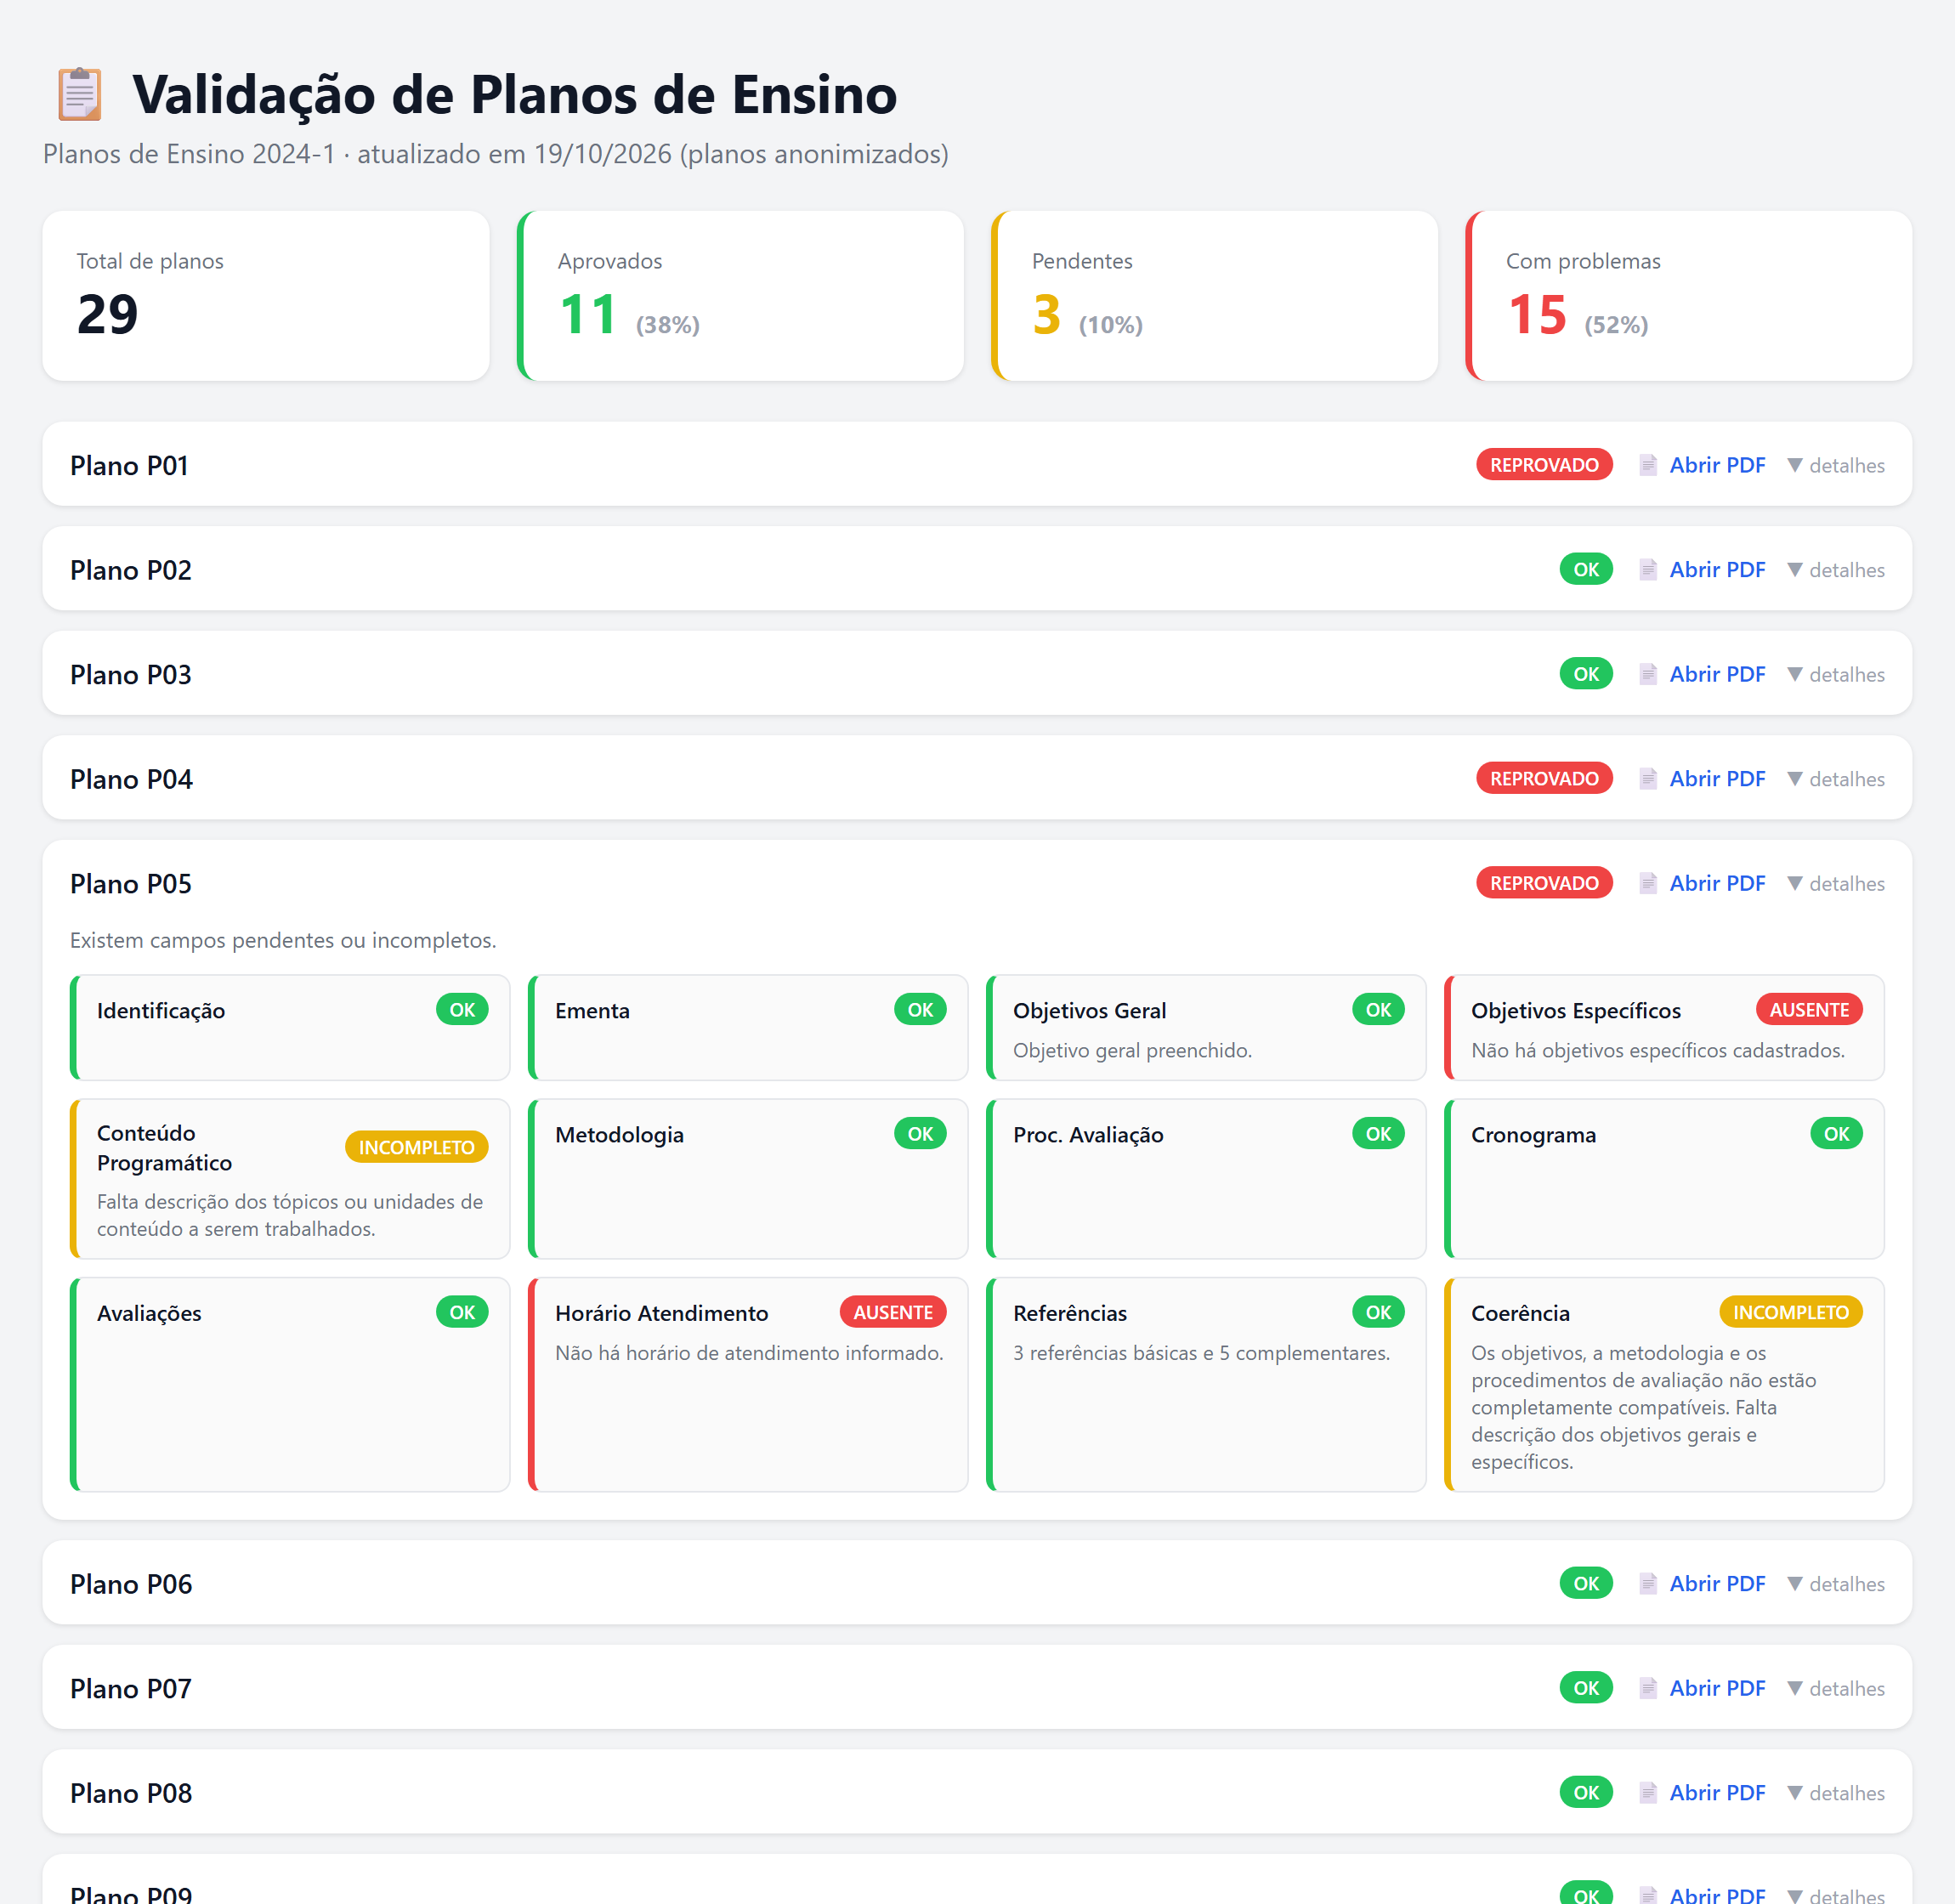
\includegraphics[width=0.92\textwidth]{images/dashboard.png}
\legend{Fonte: Elaborado pelo autor (2026). Nomes dos arquivos substituídos por códigos para anonimização.}
\end{figure}

O plano P05, expandido na figura, ilustra o uso pretendido: o avaliador vê imediatamente que faltam o horário de atendimento e os objetivos específicos e que o conteúdo programático está incompleto, e pode abrir o PDF para confirmar. O mesmo exemplo revela também uma limitação discutida na Seção \ref{sec:res-erros}: o objetivo geral aparece como OK, embora o campo contenha apenas o texto provisório ``Não Cadastrado!'' do SIGAA.

\section{Testes}
\label{sec:testes}

Para garantir que cada etapa descrita neste capítulo funcionasse como esperado ao longo das iterações, a estratégia de testes combinou três abordagens. Os testes de execução, feitos a cada alteração de um nó, usaram o modo de execução manual do n8n, que exibe a entrada e a saída de cada nó e permite inspecionar o resultado da extração, da segmentação, do \textit{prompt} e da resposta do modelo para um plano específico. Os testes de regressão, feitos ao fim de cada iteração, consistiram em processar novamente o corpus completo e comparar os resultados com os da execução anterior, verificando se a correção resolvia o problema visado sem introduzir novos erros. Por fim, a avaliação da versão final, segundo o protocolo da Seção \ref{sec:protocolo}, mediu robustez, desempenho e concordância. Os resultados dessas avaliações são apresentados no Capítulo \ref{cap:resultados}.
